\section{Benchmark PDE Problems and A Priori Spectral Analysis}
\label{sec:problems}

Before training any neural network, the singular-value decay of the training snapshots and the projection floors $\varepsilon_{\mathrm{proj}}(K)$ already establish what a linear modal reconstructor can and cannot achieve on each PDE. In this section we specify the governing equations, discretisations, loss functions, and canonical architectures of the three benchmark problems from Regazzoni et al.~\cite{regazzoni2024learning}, and we present their a priori spectral decomposition.

\subsection{The Three Benchmark Problems}

\paragraph{Test Case A: 1D Periodic Linear Advection--Diffusion--Reaction (\texttt{ADR-1b}).}
The first benchmark models a scalar concentration field $y(x,t) \in \R$ on the periodic domain $x \in [-1, 1)$ over $t \in [0, 10]$, governed by a linear advection--diffusion--reaction equation driven by a time-varying sinusoidal source whose amplitude $A(t)$ and phase shift $P(t)$ vary in time:
\begin{equation}
  \frac{\partial y}{\partial t} + c\,\frac{\partial y}{\partial x} - \mu_1\,\frac{\partial^2 y}{\partial x^2} + \mu_3\,y = A(t)\cos\!\big(\pi x - P(t)\big), \qquad x \in [-1, 1), \quad t \in (0, 10],
  \label{eq:caseA_pde}
\end{equation}
with periodic boundary conditions and homogeneous initial condition $y(x,0) = 0$. The external input signal is the two-dimensional vector $\mathbf{u}(t) = [A(t), P(t)]^\top \in \R^2$. Because the differential operator $\mathcal{L} = c\,\partial_x - \mu_1\,\partial_{xx} + \mu_3$ is linear with constant coefficients and the forcing $A(t)\cos(\pi x - P(t)) = A(t)\cos P(t)\,\cos(\pi x) + A(t)\sin P(t)\,\sin(\pi x)$ excites exclusively the fundamental wavenumber $k = 1$, every solution starting from rest lies \emph{analytically} inside the two-dimensional linear subspace $\operatorname{span}\{\cos(\pi x), \sin(\pi x)\}$:
\begin{equation}
  y(x,t) = a(t)\cos(\pi x) + b(t)\sin(\pi x).
  \label{eq:caseA_exact_span}
\end{equation}
The spatial grid comprises $N_h = 100$ uniform periodic nodes ($h = 0.02$), and trajectories are resampled linearly to $N_t = 201$ instants ($\Delta t = 0.05$). All $N_x = 100$ spatial points are used during training. The dataset is split into $100$ training, $100$ validation, and $100$ test trajectories. The canonical LDNet architecture uses a two-hidden-layer dynamics network of width $10$ ($10\text{--}10\text{--}d_s$) and a two-hidden-layer reconstructor of width $7$ ($7\text{--}7\text{--}1$, having $P_{\mathrm{rec}} = 92$ parameters at the canonical latent dimension $d_s = 2$), trained with MSE loss plus Tikhonov weight decay $\alpha_{\mathrm{reg}} = 10^{-5}$. Case~A serves as our exact-modal control: because the true manifold is strictly two-dimensional and linear in the Fourier basis, any failure of a linear reconstructor here must be attributed to coordinate mismatch or optimization rather than spatial approximation capacity.

\paragraph{Test Case B: 2D Incompressible Navier--Stokes in a Lid-Driven Cavity (\texttt{2D-Stokes}).}
The second benchmark (stored in the repository folder \texttt{2D-Stokes/}, corresponding to \texttt{src/TestCase\_2.py}) solves the full two-dimensional unsteady, incompressible Navier--Stokes equations for the velocity vector field $\mathbf{v}(\mathbf{x},t) = (v_x, v_y)^\top \in \R^2$ and pressure $p(\mathbf{x},t)$ inside the square lid-driven cavity $\Omega = [0,1]^2$:
\begin{equation}
  \begin{dcases}
    \frac{\partial \mathbf{v}}{\partial t} + (\mathbf{v}\cdot\nabla)\mathbf{v} - \nu\Delta\mathbf{v} + \nabla p = \mathbf{0}, & \text{in } \Omega \times (0, T], \\
    \nabla \cdot \mathbf{v} = 0, & \text{in } \Omega \times (0, T], \\
    \mathbf{v}(\mathbf{x},t) = \big(u(t),\,0\big)^\top \text{ on } \Gamma_{\mathrm{top}}, \qquad \mathbf{v}(\mathbf{x},t) = \mathbf{0} \text{ on } \partial\Omega \setminus \Gamma_{\mathrm{top}}, & \mathbf{v}(\mathbf{x},0) = \mathbf{0},
  \end{dcases}
  \label{eq:caseB_pde}
\end{equation}
where the time-varying top-lid horizontal velocity $u(t) \in \R$ drives Reynolds numbers up to $\mathrm{Re} \approx 1500$. Although the full-order finite element solver operates on an unstructured triangular mesh, the stored snapshots are interpolated onto a uniform $100 \times 100$ Cartesian grid ($N_h = 10{,}000$ grid nodes, spacing $\Delta x = \Delta y = 1/99$). During training and validation, only $N_x = 200$ randomly subsampled spatial points per snapshot $(s,t_i)$ are evaluated in the loss, whereas test metrics are evaluated on the full $10{,}000$-point grid. Crucially, the training ($S=80$) and validation ($S=20$) trajectories span $T = 20$ ($N_t = 101$, $\Delta t = 0.2$, $\Delta t_{\mathrm{ref}} = 5.4$), whereas the $S_{\mathrm{test}} = 10$ test trajectories span $T = 40$ ($N_t = 201$), so that the second half of every test trajectory ($t \in [20, 40]$) tests \textbf{long-time temporal extrapolation}.

Because standard MSE underweights weak recirculation vortices near the bottom corners of the cavity, the training loss augments the velocity MSE with a normalized velocity-direction penalty weighted by $0.1$ (and no Tikhonov regularisation, $\alpha_{\mathrm{reg}} = 0$):
\begin{equation}
  \mathcal{L}_{\mathrm{B}}(\hat{\mathbf{v}}, \mathbf{v}) = \operatorname{MSE}(\hat{\mathbf{v}}, \mathbf{v}) + 0.1\,\operatorname{MSE}\!\big(\mathbf{d}(\hat{\mathbf{v}}),\, \mathbf{d}(\mathbf{v})\big), \qquad
  \mathbf{d}(\mathbf{v}) = \frac{\mathbf{v}}{10^{-4} + \norm{\mathbf{v}}_2}.
  \label{eq:caseB_loss}
\end{equation}
The canonical LDNet architecture has $n^* = 1$ latent state (with $n \in \{1,5,10\}$ also explored in~\cite{regazzoni2024learning}), a two-hidden-layer dynamics network of width $w^* = 7$ ($7\text{--}7\text{--}d_s$ on $[\mathbf{s}; u]$, $P_{\mathrm{dyn}} = 85$ at $n^*=1$), and a four-hidden-layer reconstructor of width $24$ ($24^4 \to 2$ on $[\mathbf{s}; u; \mathbf{x}]$ followed by the cubic tail-compression link $\sigma_{\mathrm{out}}(o) = (o^3 + 0.05\,o)/1.05$, giving $P_{\mathrm{rec}} = 1970$ at $n^*=1$).

\paragraph{Test Case C: 1D Monodomain Aliev--Panfilov Cardiac Electrophysiology (\texttt{AP1D}).}
The third benchmark (\texttt{src/TestCase\_3.py}, located in \texttt{RQ2/AP1D/} and \texttt{RQ2-bis/ADR-1b/}) models the propagation and collision of action-potential depolarisation waves along a 1D cardiac fibre $\Omega = [0, 100]$ over $T = 500$~ms ($N_t = 501$, $\Delta t = 1$~ms, $\Delta t_{\mathrm{ref}} = 205$), governed by the dimensionless Aliev--Panfilov reaction--diffusion system~\cite{aliev1996simple} coupling the transmembrane potential $y(x,t) \in [0, 1.2]$ and a slow recovery variable $v(x,t)$:
\begin{equation}
  \begin{dcases}
    \frac{\partial y}{\partial t} - D\,\frac{\partial^2 y}{\partial x^2} + k\,y(y - a)(y - 1) + y\,v = I_{\mathrm{app}}(x,t), & x \in (0, 100), \quad t \in (0, 500], \\
    \frac{\partial v}{\partial t} = \epsilon(y,v)\,\big(-v - k\,y(y - a - 1)\big), & \frac{\partial y}{\partial x}(0,t) = \frac{\partial y}{\partial x}(100,t) = 0,
  \end{dcases}
  \label{eq:caseC_pde}
\end{equation}
starting from the unexcited rest state $y(x,0) = 0, v(x,0) = 0$. The external input $\mathbf{u}(t) = [I_{\mathrm{app},1}(t), I_{\mathrm{app},2}(t)]^\top \in \R^2$ consists of two localized stimulus pulse trains applied near the two ends of the fibre, which trigger steep travelling depolarisation fronts that propagate inward, collide, annihilate, and undergo slow repolarisation. The spatial grid has $N_h = 101$ uniform nodes ($h = 1$, subsampled by a factor of $8$ from the $801$-node FOM mesh), with $N_x = 20$ random spatial points per $(s,t_i)$ used during training and validation, and all $101$ points evaluated at test time across $100$ training, $100$ validation, and $200$ test trajectories. The canonical LDNet uses $n^* = 12$ latent states, a single-hidden-layer dynamics network of width $w^* = 8$ ($8\text{--}d_s$ on $[\mathbf{s};\mathbf{u}]$ with the exact rest-state equilibrium subtraction~\eqref{eq:equilibrium_offset}, $P_{\mathrm{dyn}} = 228$ at $n^*=12$), and a five-hidden-layer reconstructor of width $17$ ($17^5 \to 1$ on $[\mathbf{s}; x]$ with no $\mathbf{u}$ input and no output link, $P_{\mathrm{rec}} = 1480$ at $n^*=12$), trained with MSE loss plus Tikhonov weight $\alpha_{\mathrm{reg}} = 4.7 \cdot 10^{-3}$ on both sub-networks.

\begin{table}[!htbp]
\centering
\caption{Summary of the three benchmark PDE problems, discretisation grids, canonical LDNet architectures, and experimental sweep factors in \texttt{RQ2} and \texttt{RQ2-bis}.}
\label{tab:benchmarks_summary}
\footnotesize\resizebox{\textwidth}{!}{%

\begin{tabular}{@{}p{3.1cm}p{3.8cm}p{4.3cm}p{4.3cm}@{}}
\toprule
\textbf{Attribute} & \textbf{Case A (\texttt{ADR-1b})} & \textbf{Case B (\texttt{2D-Stokes})} & \textbf{Case C (\texttt{AP1D})} \\
\midrule
Governing physics & 1D periodic linear ADR with sinusoidal forcing & 2D incompressible Navier--Stokes lid-driven cavity ($\mathrm{Re}\lesssim 1500$) & 1D Aliev--Panfilov excitable tissue (travelling fronts \& collisions) \\
Spatial grid \& BCs & $N_h = 100$ on $[-1,1)$, $h=0.02$, periodic & $N_h = 100\times 100$ on $[0,1]^2$, $h=1/99$, Dirichlet no-slip/lid & $N_h = 101$ on $[0,100]$, $h=1$, homogeneous Neumann \\
Training subsample $N_x$ & All $100$ points & $200$ random pts per $(s,t_i)$ & $20$ random pts per $(s,t_i)$ \\
Time grid \& horizon & $\Delta t = 0.05$, $N_t = 201$, $T = 10$ & $\Delta t = 0.2$, $\Delta t_{\mathrm{ref}}=5.4$; train/val $T=20$ ($N_t=101$), test $T=40$ ($N_t=201$) & $\Delta t = 1$~ms, $\Delta t_{\mathrm{ref}}=205$; $T=500$~ms ($N_t=501$) \\
Splits (train / val / test) & $100$ / $100$ / $100$ & $80$ / $20$ / $10$ & $100$ / $100$ / $200$ \\
Input signal $\mathbf{u}(t)$ & $[A(t), P(t)]^\top \in \R^2$ & Lid velocity $u(t) \in \R^1$ & Stimulus pulses $[I_1(t), I_2(t)]^\top \in \R^2$ \\
Decoder input $\mathbf{z}(t)$ & $\mathbf{s}(t) \in \R^{d_s}$ ($r=d_s$) & $[\mathbf{s}(t); u(t)] \in \R^{d_s+1}$ ($r=d_s+1$) & $\mathbf{s}(t) \in \R^{d_s}$ ($r=d_s$) \\
Loss function & $\mathrm{MSE} + 10^{-5}\norm{\theta}_2^2$ & $\mathrm{MSE}(\mathbf{v}) + 0.1\,\mathrm{MSE}(\mathbf{d}(\mathbf{v}))$, $\alpha_{\mathrm{reg}}=0$ & $\mathrm{MSE}(y) + 4.7\cdot 10^{-3}\norm{\theta}_2^2$ \\
Ratio $\NRMSE / \varepsilon_{\mathrm{total}}$ & $c_A = 0.16857$ & $c_B = 0.04796$ & $c_C = 0.34836$ \\
 Relative mean $\frac{\mathrm{rms}(\bar{y})}{\mathrm{rms}(y)}$ & $0.520$ & $0.175$ & $0.481$ \\
Canonical latent $d_s^*$ ($n^*$) & $2$ & $1$ (paper also tests $5, 10$) & $12$ \\
Canonical $\NNdyn$ ($w^*, L^*$) & $10\text{--}10\text{--}d_s$ ($w^*=10, L^*=2$) & $7\text{--}7\text{--}d_s$ ($w^*=7, L^*=2$, $P_{\mathrm{dyn}}=85$ at $n^*=1$) & $8\text{--}d_s$ with eq.\ offset ($w^*=8, L^*=1$, $P_{\mathrm{dyn}}=228$ at $n^*=12$) \\
Canonical $\mathrm{L0}$ $\NNrec$ & $7\text{--}7\text{--}1$ ($P_{\mathrm{rec}}=92$ at $d_s^*=2$) & $24^4\to 2$ + cubic link ($P_{\mathrm{rec}}=1970$ at $n^*=1$) & $17^5\to 1$, no link ($P_{\mathrm{rec}}=1480$ at $n^*=12$) \\
Modal basis $\{\varphi_k\}$ & Orthonormal Fourier & Discrete vector POD on $(v_x,v_y)$ & Trapezoidal-QR Legendre \\
\texttt{RQ2} budget \& runs & 50 Adam + 150 BFGS (348 runs) & 200 Adam + 500 BFGS (195 runs) & 200 Adam + 500 BFGS (273 runs) \\
\texttt{RQ2-bis} budget \& runs & Not run (already converged in \texttt{RQ2}) & 0 Adam + $10{,}000$ BFGS (63 cluster + 63 laptop runs) & 0 Adam + $10{,}000$ BFGS (63 cluster + 63 laptop runs) \\
\bottomrule
\end{tabular}
}
\end{table}

\subsection{A Priori Singular-Value Decay and Projection Floors Before Training}
\label{sec:spectra_and_floors}

Figure~\ref{fig:rq2_fig1} and Table~\ref{tab:projection_floors} display the normalised singular values $\sigma_k/\sigma_1$ of the centred training snapshot matrix (left panel, serving as an empirical proxy for the Kolmogorov $n$-width decay) and the relative projection floors $\varepsilon_{\mathrm{proj}}(K)$ evaluated on the test set for both the protocol basis $\{\varphi_k\}$ and the optimal training POD basis (centre and right panels).

\begin{figure}[!htbp]
  \centering
  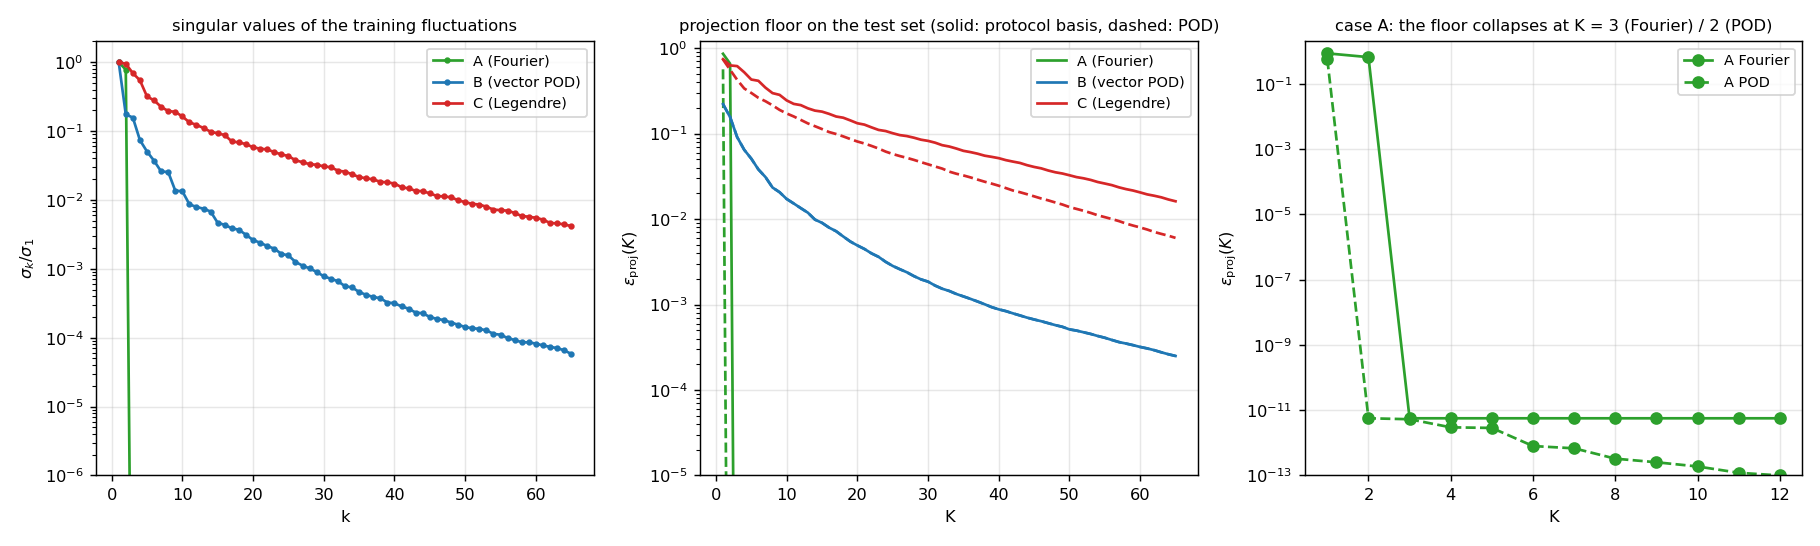
\includegraphics[width=0.90\textwidth,height=0.215\textheight,keepaspectratio]{fig1_spectra_floors.png}
  \caption{A priori spectral characterization of the three PDE benchmarks before any neural network training. \textbf{Left:} singular values $\sigma_k/\sigma_1$ of the centred training snapshots (empirical Kolmogorov $n$-width decay). \textbf{Centre:} test-set projection floor $\varepsilon_{\mathrm{proj}}(K)$ for the protocol basis (solid: Fourier in A, vector POD in B, discrete-QR Legendre in C) and for the optimal empirical POD basis (dashed). \textbf{Right:} zoom on Case~A, where the projection floor drops to numerical round-off ($\sim 6\cdot 10^{-12}$) at $K=2$ for POD and $K=3$ for Fourier (whose first mode $1/\sqrt{2}$ is constant).}
  \label{fig:rq2_fig1}
\end{figure}

\begin{table}[!htbp]
\centering
\caption{Test-set relative projection floor $\varepsilon_{\mathrm{proj}}(K) = \norm{(y-\bar{y}) - P_K(y-\bar{y})}_w / \norm{y}_w$ across modal truncation levels $K$ for the protocol basis and the empirical training POD basis. Multiply by $c_A = 0.1686$, $c_B = 0.0480$, or $c_C = 0.3484$ to convert $\varepsilon_{\mathrm{proj}}(K)$ into test $\NRMSE$.}
\label{tab:projection_floors}
\small\resizebox{\textwidth}{!}{%

\begin{tabular}{@{}rlllll@{}}
\toprule
\textbf{Modes $K$} & \textbf{Case A (Fourier)} & \textbf{Case A (POD)} & \textbf{Case B (Vector POD)} & \textbf{Case C (Legendre)} & \textbf{Case C (POD)} \\
\midrule
$1$  & $0.8596$ & $0.5649$ & $0.2215$ & $0.7432$ & $0.7371$ \\
$2$  & $0.6581$ & $5.66\cdot 10^{-12}$ & $0.1563$ & $0.6280$ & $0.5587$ \\
$3$  & $5.66\cdot 10^{-12}$ & $5.30\cdot 10^{-12}$ & $0.0910$ & $0.6166$ & $0.4261$ \\
$5$  & $5.66\cdot 10^{-12}$ & $2.87\cdot 10^{-12}$ & $0.0509$ & $0.4294$ & $0.2991$ \\
$9$  & $5.66\cdot 10^{-12}$ & $2.55\cdot 10^{-13}$ & $0.0206$ & $0.2841$ & $0.1895$ \\
$10$ & $5.66\cdot 10^{-12}$ & $1.89\cdot 10^{-13}$ & $0.0172$ & $0.2447$ & $0.1721$ \\
$12$ & $5.66\cdot 10^{-12}$ & $1.00\cdot 10^{-13}$ & $0.0134$ & $0.2155$ & $0.1447$ \\
$17$ & $5.66\cdot 10^{-12}$ & $2.53\cdot 10^{-14}$ & $0.00721$ & $0.1585$ & $0.0989$ \\
$33$ & $5.66\cdot 10^{-12}$ & $2.39\cdot 10^{-15}$ & $0.00144$ & $0.0706$ & $0.0359$ \\
$65$ & $5.66\cdot 10^{-12}$ & $1.24\cdot 10^{-15}$ & $2.50\cdot 10^{-4}$ & $0.0162$ & $0.00603$ \\
\midrule
Smallest $K$ for $\varepsilon_{\mathrm{proj}} \le 10\%$ & $3$ & $2$ & $3$ & $26$ & $17$ \\
Smallest $K$ for $\varepsilon_{\mathrm{proj}} \le 5\%$  & $3$ & $2$ & $6$ & $41$ & $28$ \\
Smallest $K$ for $\varepsilon_{\mathrm{proj}} \le 1\%$  & $3$ & $2$ & $14$ & $>65$ & $57$ \\
\bottomrule
\end{tabular}
}
\end{table}

Table~\ref{tab:projection_floors} reveals three sharply contrasting approximation regimes:
\begin{enumerate}[leftmargin=2em]
  \item \textbf{Case A is finite-rank and exactly modal:} Only two singular values are non-zero ($\sigma_2/\sigma_1 = 0.78$, $\sigma_3/\sigma_1 \approx 10^{-11}$). Because the protocol orders the Fourier basis starting with the spatially constant mode $\varphi_1(x) = 1/\sqrt{2}$ (which carries zero energy once the zero-wavenumber mean field is subtracted), $K=2$ spans $\{1/\sqrt{2}, \cos(\pi x)\}$ and omits $\sin(\pi x)$ ($\varepsilon_{\mathrm{proj}}(2) = 0.658$). At $K=3$, both $\cos(\pi x)$ and $\sin(\pi x)$ are included and $\varepsilon_{\mathrm{proj}}(K)$ collapses to $5.66\cdot 10^{-12}$ for all $K \ge 3$.
  \item \textbf{Case B exhibits rapid exponential POD decay:} Despite the nonlinear convective term $(\mathbf{v}\cdot\nabla)\mathbf{v}$ and the lid-corner velocity discontinuities, the cavity flow is confined to a fixed geometry where viscosity smooths the interior vorticity field. The singular values decay geometrically as $\sigma_k/\sigma_1 \sim e^{-0.1 k}$ ($\sigma_2/\sigma_1 = 0.175$, $\sigma_5/\sigma_1 = 0.050$, $\sigma_{10}/\sigma_1 = 0.013$, $\sigma_{17}/\sigma_1 = 0.0039$, $\sigma_{65}/\sigma_1 = 5.8\cdot 10^{-5}$). Just $K=6$ POD modes capture $95\%$ of the relative field norm ($\varepsilon_{\mathrm{proj}}(6) \le 0.05$, corresponding to $\NRMSE \le 2.4\cdot 10^{-3}$), $K=17$ modes give $\varepsilon_{\mathrm{proj}}(17) = 7.21\cdot 10^{-3}$ ($\NRMSE = 3.46\cdot 10^{-4}$), and $K=65$ modes give $\varepsilon_{\mathrm{proj}}(65) = 2.50\cdot 10^{-4}$ ($\NRMSE = 1.20\cdot 10^{-5}$). Thus, linear spatial reconstruction is not a bottleneck in Case~B.
  \item \textbf{Case C exhibits the classic Kolmogorov $n$-width barrier of travelling fronts:} The leading singular values remain nearly flat ($\sigma_2/\sigma_1 = 0.94$, $\sigma_3/\sigma_1 = 0.69$, $\sigma_5/\sigma_1 = 0.32$, $\sigma_{10}/\sigma_1 = 0.16$), and between $k=10$ and $k=65$ they decay by a factor of only $39$ (compared with $230$ in Case~B). Reaching a $5\%$ relative projection floor requires $K = 28$ optimal POD modes or $K = 41$ Legendre polynomials; at $K = 33$, the Legendre floor is still $\varepsilon_{\mathrm{proj}}(33) = 0.0706$ ($\NRMSE = 2.46\cdot 10^{-2}$), and even for an ideal $12$-dimensional linear subspace ($d_s^* = 12$), the POD rank floor is $\varepsilon_{\mathrm{rank}}(12) = 0.1447$ ($\NRMSE = 5.04\cdot 10^{-2}$).
\end{enumerate}
Crucially, projection floors provide \textbf{necessary} conditions for accuracy, never sufficient ones: they prove a priori that no linear decoder with $d_s \le 12$ can reach $\NRMSE < 5\cdot 10^{-2}$ in Case~C, whereas whether a modal decoder can actually approach its tiny floor in Case~B depends on the latent dynamics $\NNdyn$ and the optimizer.
